%************************************************
\chapter{Metacognition}\label{ch:metacognition}
%************************************************

% Intro
\begin{flushright}{\slshape
    The world is my idea. \\
    --- A. Shopenhauer \cite{schopenhauer_world_2016}}
\end{flushright}
As many insightful people before him, Shopenhauer recognized that we all see the world through our own personal lenses of perception. His original words "Die Welt ist meine Vorstellung" are sometimes translated as "the world is my \emph{representation}", which should sound more familiar to a modern-day cognitive scientist. Indeed, behaviors we observe in humans and other animals are caused by idiosyncratic chains of neurophysiological events assumed to implement functional computations from certain inputs to certain outputs. Intermediate stages of these computations feature interactions between representations: of various external and internal variables, and of current goals and needs. In this chapter, I explore how the representation of \acf{LP} might form and manifest inside the human mind. 

% Quick recap of evidence for learning progress
Previously, I discussed the idea that information-seeking is motivated by expected improvement of knowledge or \ac{LP}. A few studies lend empirical support for this theory by measuring various task features and examining their relationships with task engagement. For example, Gerken et al. \cite{gerken_infants_2011} measured objective complexity of experimental stimuli and tested its relationship with attention. Poli et al. \cite{poli_infants_2020} made a step further by proposing several candidate mechanisms processed stimuli of different complexity and examining how their outputs related to looking time. Leonard et al. \cite{leonard_young_2021} manipulated performance feedback to control how children perceived their task progression and observed whether they were willing to carry on. Son and Metcalfe \cite{son_metacognitive_2000} asked university students to report how well they thought they would remember information from different texts and looked at how well these reports predicted time allocation and prioritization of these texts. In our own study \cite{ten_humans_2021}, we manipulated the complexity of categorization rules of different stimulus families and measured people's ongoing performance to understand its relation to self-directed learning. While these studies suggest different ways to measure \ac{LP}, they do not make explicit claims about the algorithmic implementation of the underlying computation.

% Prospective vs retrospective judgments
It is important to note that the studies reviewed above are concerned with how \emph{prospective} \ac{LP} judgments influence motivation. How such \ac{LP} expectations arise is beyond the scope of this chapter, because there are probably many variables and processes that jointly determine people's expectations about their future learning and achievement. A relevant framework for exploring the mechanisms of prospective \ac{LP} expectations is Bandura's theory of \emph{self-efficacy} \cite{bandura_self-efficacy_1977}. Bandura proposed several qualitatively different sources that contribute to one's belief about being able to perform a task, including (1) performance accomplishments, (2) vicarious experiences, (3) verbal persuasion, and (4) emotional arousal. The present chapter is concerned with a single part of this belief-formation process: the subjective evaluation of one's learning/performance dynamics. 

% Motivation and goals
What information does the human brain access and represent in order to compute the \ac{LP} on a given task? Computational literature proposes several operational mechanisms \cite{oudeyer_what_2007,graves_automated_2017,twomey_curiosity-based_2018,linke_adapting_2020}. All of these mechanisms assume an interaction between two distinct functional components, or modules. One module -- let's call it the \emph{task module} -- is a mechanism that learns to perform a task at hand. It serves to convert sensory/mnemonic inputs into response outputs (e.g., motor action, categorization, etc.). The second module -- the \emph{meta-module} -- serves to evaluate the task module in order to inform decisions pertaining to active learning and/or task selection. The meta-module performs some kind of differentiation of the task module's performance in order to generate the \ac{LP} signal.  

% A taxonomy
Despite the similarities, we can identify two fairly distinct families of mechanisms. The first one -- called \emph{performance-based mechanisms} -- assumes that the meta-module computes \ac{LP} based on the task module's performance. Here, the task module is essentially a blackbox and the meta-module's job is to infer how this blackbox learns by observing its behavior. The second family -- \emph{introspective mechanisms} -- assumes that \ac{LP} is computed by observing the structural changes in the task module itself. Here, the meta-module has elevated access to the task module's inner structure, which allows it to observe and quantify changes in the task module as it learns its task.

\section{Mechanisms of Progress Computation}

\subsection{Performance-based Mechanisms}\label{subsec:performance-based_mechanisms}

% Schmidhuber (1991)
A commonly used approach to estimating \ac{LP} in \ac{AI}, is to compute a temporal derivative of the task module's performance trajectory. Computational architectures of intrinsically-motivated exploration provide numerous examples of how such computations can be carried out and what information needs to be represented to support them. An early algorithm by Schmidhuber \cite{schmidhuber_curious_1991} estimates \ac{LP} as:
\begin{equation}
    \mathrm{LP(t)} = o_C(t) - o_C'(t)
\end{equation}
where $o_C(t)$ is an estimated reliability of the task module -- or the "confidence" at time $t$ of the meta-module in the competence of the task module; the term $o_C'(t)$ denotes the reliability estimate after the meta-module had been adjusted to predict the reliability of the task module more accurately. Here, \ac{LP} is computed by comparing point estimates of subjective confidence before and after updating the meta-module with relevant information. As per Schmidhuber's original proposition, this information can be derived by counting how many times the task in a given context was performed well and how many times the task was attempted in this context.

% Oudeyer, Kaplan, & Hafner (2007)
In a different algorithm by Oudeyer, Kaplan, and Hafner \cite{oudeyer_intrinsic_2007} \ac{LP} is defined as:
\begin{equation}
    \mathrm{LP(t)} = e_R(t) - e_R(t-\tau)
\end{equation}
where $e_n(t)$ is the average prediction error of the task module prior to time $t$; the parameter $\tau$ controls the temporal reference point to which $e_n(t)$ is compared. The original algorithm also parameterizes the computation of the prediction-error averages to control their smoothness. Importantly, \ac{LP} is computed separately for different regions, indexed by $R$, of the sensorimotor space to prevent the agent from "maximizing" progress by alternating between attempting unrelated low- and high-error tasks in an undifferentiated space. Like in Schmidhuber's algorithm, the mean error term $e_n(t)$ can also be construed as the meta-module's confidence in the task module, as it represents the error rate in a given context. 

% Colas et al. (2019), Baranes & Oudeyer (2013)
Similar algorithms have been used to compute competence progress \cite{baranes_active_2013,santucci_which_2013,colas_curious_2019,forestier_intrinsically_2020} -- a temporal derivative of the agent's ability to reach its goals in a specific task space. For instance, Colas et al. \cite{colas_curious_2019} defined \ac{LP} as:
\begin{equation}
    \mathrm{LP(n)} = |c_R(n) - c_R(n-\tau)|
\end{equation}
where $c_R(n)$ is the subjectively estimated competence of the agent in a discrete task space, indexed by $R$; $n$ is the number of self-evaluations performed to estimate the competence score. Subjective competence is evaluated by weighting binary goal-achievement outcomes in a task space by recency and taking the average of the weighted scores\footnote{Colas et al. \cite{colas_curious_2019} used a queue-based implementation, but the effect of the computation is the same as taking a recency-weighted average of a binary vector.}. Competence is computed for all $n$ self-evaluation trials and again for a more recent $n-\tau$ portion of these trials, and the two estimates are compared. Note that here, the absolute value of the derivative is taken. While not essential to the definition of \ac{LP}, this functional form raises the question of whether improvement and deterioration in performance are equivalent for motivation and what their differences might be. In Colas et al. \cite{colas_curious_2019}, taking the absolute value of the competence differential allowed the agent to actively practice tasks on which it was getting worse over time, which ensured that the overall competence was maximized.

% The significance of uncertainty
In the approaches discussed above, the represented measure of performance can be thought of as reflecting the agent's subjective belief about its performance, suggesting that changes in subjective beliefs might underlie \ac{LP} computation. However, the above mechanisms rely on point-estimate representations that do not account for belief uncertainty. On the other hand, psychological literature suggests that declarative statements (e.g., "I can play the piano") emerge from supporting representations of varying degrees of internal consistency \cite{smith_belief_1991,koriat_self-consistency_2012}. More recently, research in neuroscience has started to unravel the neural mechanisms underlying uncertainty and confidence judgments. The so-called distributional uncertainty inherent in neural activity can potentially explain how the brain computes and represents propositional confidence \cite{meyniel_confidence_2015,pouget_confidence_2016}. If the computation of \ac{LP} involves belief comparison, then belief uncertainty should have a considerable footprint on the process. 

% Bayesian beliefs, uncertainty and confidence
A suitable tool for studying dynamic uncertain beliefs is the Bayesian framework for cognitive modeling, which assumes that humans represent beliefs probabilistically \cite{sun_bayesian_2008,perfors_tutorial_2011,coenen_asking_2019}. Sensitivity to uncertainty enables agents to intelligently switch between exploration and exploitation \cite{cohen_should_2007} and control the learning of new information \cite{meyniel_confidence_2015}. In addition to uncertainty inherent in belief distributions, individual beliefs (that a particular decision or proposition is true) are associated with a distinct kind of uncertainty that manifests in confidence judgments \cite{pouget_confidence_2016}. Confidence in beliefs is often sufficient to support decisions and might be a simplified computational substitute for overly complex belief posteriors \cite{pouget_confidence_2016}.  

% Formal description
Probabilistic beliefs (that one can accomplish a task) can be characterized by more or less confidence and change as a result of self-monitoring. The evolution of such beliefs can be expressed in terms of posterior probability. For example, suppose that an agent represents a state space, a subset of which is a state-achievement event $A$ that has a probability of occurring, $P(A)$. This probability can be framed as the subjective belief that event $A$ can be reached by the agent; we might as well call it the agent's confidence in achieving $A$. Confidence can be updated by observing a history of state-achievement events from the past $D$:
\begin{equation}
    P(A|D) = \frac{P(D|A) P(A)}{P(D|A)P(A) + P(D|A^c)P(A^c)}
\end{equation}
where $A^c$ denotes the complement of $A$. This equation prescribes an optimal way to update a binary state-achievement belief by combining the prior expectation $P(A)$ with the normalized likelihood of that belief $P(D|A)$. Both of these components reflect the agent's uncertain knowledge about its abilities to predict the future or reach specific goal states.

% Prior knowledge
Note how the prior confidence $P(A)$ biases how the observed data influences the posterior. For example, imagine that while estimating confidence, all that the agent observes is external binary feedback on some goal-achievement task. Now, consider the following priors and likelihood values:
\begin{center}
\begin{tabular}{c c c c}
Belief & $P(A)$ & $P(D=\mathrm{success}|A)$ & $P(D=\mathrm{fail}|A)$ \\ 
$A$    & .99    & .90                       & .10        \\  
$A^c$  & .01    & .05                       & .95         
\end{tabular}
\end{center}
The posterior from a 'success' outcome will be .9994 (an increase of .0094), while a 'fail' outcome will give us a posterior of .9124 (a decrease of .0776). Thus, high prior confidence in accomplishing the task results in asymmetric updates for different outcomes. Incidentally, the surprise from observing a failure while strongly expecting success is much higher than the surprise from observing success. The strong-expectation prior can be contrasted with the maximally uncertain prior, $P(A) = .5$: the posteriors will change by +.45 and -.40, for 'success' and 'fail' outcomes, respectively. In this case, the update is larger and relatively less asymmetric. Such dynamics are not captured by point-estimate heuristic methods.

% Alternative computation of binary beliefs
Note that to compute the posterior $P(A|D)$, the agent needs to represent a contingency table of all their attempts. This entails storing the counts of successes and failures across beliefs that assume that $A$ can and cannot be reached. An alternative approach is to represent confidence as the parameter $q$ of the Bernoulli distribution, therefore, $P(A|q) = q$. This way, confidence itself is an uncertain quantity that can be shaped by the data:
\begin{equation}
    p(q|D) = \frac{P(D|q) p(q)}{\int_{0}^{1}P(D|q)p(q)dq}
\end{equation}
To update the prior $p(q)$, it suffices to remember the binary outcomes of the most recent attempt, since the likelihood can be computed from $q$ alone: $P(D|q) = q^D(1-q)^{(1-D)}$. Assuming that $p(q)$ is given by the Beta distribution, we get a well-known Beta-Binomial Bayesian model that can be readily applied empirical data to test assumptions about prior expectations and confidence updating.

% When external binary feedback is not available
In the simple examples above, the agent only considers binary feedback data to update its beliefs. While performance feedback affects subjective confidence judgments \cite{marti_certainty_2018,rouault_forming_2019}, other factors relating to task performance might be at play, especially when reliable external feedback is absent or very sparse \cite[e.g.,][]{rouault_forming_2019,holm_episodic_2019,locke_performance_2020}. For instance, when trying to answer a question, one might consider the utility of self-generated candidate answers \cite{coenen_asking_2019} in order to gauge how close one is to answering. In a visuomotor task of tracking the center of a dot-cloud \cite{locke_performance_2020}, participants monitored the distance between the invisible target and the cursor to make judgments about their performance. Such continuous evaluations are useful for assessing one's progress when external feedback is not available. This implies that feelings of progress may be supported not only by monitoring the success rate but also the proximity to success.

% A note on IM RL
The problem of lacking reliable feedback is at the heart of intrinsically motivated machine learning \cite{oudeyer_computational_2018,linke_adapting_2020} where the proposed solution is to provide the agent with intrinsic reward functions that support learning in the absence of primary rewards. Such intrinsic reward functions, however, are usually characterized as task-independent and are intended to enhance the agent's competence in a general way. Evaluation of the proximity to task achievement discussed here, on the other hand, is tied to the task itself.

% A sketch for a competence proxy computation
The nature of information that contributes to task-achievement proximity depends on the task and how agents represent achievement (or goals). To illustrate, consider the following example. We know that a skillful bow-and-arrow shooter is one that tends to hit the target within the bullseye region. Before ever hitting the sweet spot, a practicing shooter might consider the distance to the target's center, $d$, in order to evaluate her ability (for simplicity, suppose that $d$ represents signed horizontal distance to the center). The learner will expect some variability in the outcomes of her attempts, e.g., $d \sim \mathcal{N}(0, \sigma)$, where the value of the variance parameter $\sigma$ is unknown a priori. Suppose that the learner can (1) represent a hypothesis about what skillful performance should be in terms of the spread of outcomes, and (2) infer her own level of performance from new observations and prior knowledge. Concretely, we can assume that skillful performance is represented by a very small amount of variability around the bullseye, i.e., $\sigma=\sigma^*$. As the learner tries to accomplish the task, she observes where she hits (or misses) the target and updates her uncertain belief about how varied her attempts tend to be. To model this belief update, we can use the Bayes rule:
\begin{equation}
    p(\sigma|d) = \frac{P(d|\sigma)p(\sigma)}{\int_{0}^{+\infty}P(d|\sigma)p(\sigma)d \sigma}
\end{equation}
where $p(\sigma)$ is the prior distribution over $\sigma$ (e.g., a conjugate inverse-gamma prior), and $P(d|\sigma)$ is the likelihood term given by the Gaussian density function with $\mu=0$ and $\sigma$. After an attempt at the task, the learner can compare the target performance ($\sigma^*$) with their actual performance. This can be achieved in several ways. For example, a summary statistic derived from the posterior (e.g., the maximum a posteriori estimate or the expected value of $\sigma$) can be compared directly with $\sigma^*$. However, in order to account for belief uncertainty, we can model the estimation of goal-proximity ($\mathrm{GP}$) as Bayesian model comparison:
\begin{equation}
   \mathrm{GP} = \log \frac{P(H_1|d)}{P(H_0|d)} = \log \frac{P(d|H_1)}{P(d|H_0)} + \log \frac{P(H_0)}{P(H_1)}
\end{equation}
where $H_0$ represents a "goal-achievement hypothesis" that $\sigma = \sigma^*$ and $H_1$ represents an "alternative hypothesis" that $\sigma$ is distributed according to $p(\sigma|d)$. Improving performance in relation to the $\sigma^*$-criterion will drive this posterior log odds towards zero. As with the feedback-based example above, this way of modeling proxy-competence takes into account the prior knowledge over the hypotheses: if the learner hits the bullseye while expecting a large spread of outcomes, they might discredit it as a lucky fluke. 

% Comparison with heuristic methods
To compute \ac{LP}, the learner would need to compare confidence or (proxy-)competence estimations at different points in time, e.g.:
\begin{equation}
   \mathrm{LP}_t = \mathrm{GP}_{t} - \mathrm{GP}_{t-\tau}
\end{equation}
where $\mathrm{GP}_t$ is the goal-proximity measure at time $t$ based on the data and prior knowledge at that point in time. We can picture a more Bayesian approach to estimating \ac{LP}. For instance, \ac{LP} can be itself represented as an inferred parameter with a prior distribution and a likelihood. 

\subsection{Introspective  Mechanisms}\label{subsec:introspective_approaches}

Introspective approaches to computing \ac{LP} are based on the model of the learning process of the task module. In contrast to the performance-based mechanisms, where the meta-module observes consequences of the task module's behavior, the introspective accounts require specifying how the task module itself adapts to its task demands. How \ac{LP} is computed depends entirely on the learning mechanism\footnote{In this particular instance, the mechanism refers to any learning rule that determines how the task module's behavior changes by data. Bayesian models of learning typically avoid implementational claims about the underlying mechanisms, yet they describe how the system's knowledge changes (or how it should change).} specified for the task module. Note that for methods reviewed in this section, the time over which \ac{LP} is computed is implicit -- a measurement is performed each time an arbitrary amount of data is processed by the task module.

% Twomey and Westerman, 2018
One example is a connectionist model of infant categorization from Twomey and Westermann \cite{twomey_curiosity-based_2018}. The model features an autoencoder neural network for compressing stimulus representations into a relatively small set of features. These compressed feature representations are not given, but have to be learned from observing stimuli -- here, instances of a latent structure. When an autoencoder "understands" the latent structure well, it can encode the full representation into a compact format and then decode it back into the full representation. Latent representations are learned by adjusting connection weights in the network via backward propagation of error -- a mismatch between the encoded and the decoded representation. Based on this architecture, Twomey and Westerman compared several intrinsic-motivation signals that could inform how the network should choose stimuli to learn from. One of the signals was the total amount of weight adaptation in the network. For a single weight connecting an input neuron to an output neuron, the update is given by: 
\begin{equation}
    \Delta w = (i - o)o(1-o)
\end{equation}
where $i$ is the target activation and $o$ is the actual activation of the output neuron. Total weight adaptation can be obtained by summing over the absolute values of individual weight updates. Since knowledge in connectionist systems resides in connection weights, this measure can be regarded as a version of \ac{LP} because weights are adjusted to minimize the network's error (i.e., improve the network's knowledge). Thus: 
\begin{equation}
    \mathrm{LP} = \sum_{w \in \bm{w}} |\Delta w|
\end{equation}
where $\bm{w}$ is a vector of all weights in the network.

% Graves et al., 2017 -- Change to variational complexity gain (a retrospective LP measure)
Another example of an introspective mechanism comes from a study by Graves and colleagues \cite{graves_automated_2017}. The authors investigated the effects of different \ac{LP} measures on automated curriculum learning -- a process by which a meta-module autonomously selects data to train the task module. The task module was a Bayesian neural network with probabilistic weight parameters \cite{blundell_weight_2015}. In contrast to traditional neural networks, Bayesian neural networks feature a multivariate parametric distribution for their connection weights. Instead of optimizing the weights themselves, Bayesian neural networks learn by optimizing distributional parameters. In \cite{graves_automated_2017}, network parameters were optimized with respect to the minimum description length objective \cite[see][]{graves_practical_2011}. Based on these specifications, one version of \ac{LP} -- called \emph{variational complexity gain} -- was defined as a decrease in model complexity:
\begin{equation}
    \mathrm{LP} = D_{\mathrm{KL}}(P_{\phi'}||Q_{\psi'}) - D_{\mathrm{KL}}(P_{\phi}||Q_{\psi})
\end{equation}
where $D_{\mathrm{KL}}(P_{\phi}||Q_{\psi})$ is the Kullback-Leibler divergence between the variational posterior distribution $P_{\phi}$ and the prior distribution $Q_{\psi}$. In the context of variational optimization of the minimum description length objective, the \ac{LP} definition from above is interpreted as model complexity gain, which occur only when data is compressed by a greater amount \cite{graves_automated_2017}. Note that in practice, this measure did not work as well as a less computationally expensive mechanism based on prospective approximations of variational complexity gains.
%-- called \emph{gradient variational complexity gain} -- was defined as a directional derivative of the Kullback-Leibler (KL) divergence (a.k.a. relative entropy) in the direction of gradient descent:
% \begin{equation}
%     \mathrm{LP} = [\nabla_{\phi,\psi} \mathrm{KL}(P_{\phi} || Q_{\psi})]^\top \nabla_{\phi} \displaystyle \mathop{\mathbb{E}}_{\theta \sim P_{\phi}} L(x, \theta)
% \end{equation}
% Details aside, this form of \ac{LP} can be interpreted as a Bayesian-neural-network a loss-reduction measure in a traditional neural network. It approximates how much the $\mathrm{KL}$ divergence between the (variational) posterior and the prior weight distributions would change if they were adjusted to optimize the likelihood of the data \cite[see][]{graves_automated_2017}.

% Poli et al., 2020
Poli et al. \cite{poli_infants_2020} studied a probabilistic model of infant attention in a task where a visual cue stochastically appeared in one of four locations according to a fixed probability distribution. Infants could learn this distribution by observing multiple trials of cue presentation, and looked away once the distribution was learned. The authors modeled the task module as a probabilistic predictor of the cue location that optimally changed its predictions on each bout of cue presentation via sequential Bayesian inference. They defined \ac{LP} as the KL divergence between the prior distribution before cue presentation and the posterior distribution after cue presentation:
\begin{equation}
    \mathrm{LP} = D_{\mathrm{KL}}(p^j||p^{j-1})
\end{equation}
where $p^j$ is the posterior distribution of the parameters determining the prediction on trial $j$. This form of \ac{LP} can be interpreted as the degree to which predictions of the task model change. Implicitly, because of the stationarity of environment and the optimality of Bayesian inference, these changes lead to more accurate predictions. Note, that this \ac{LP} measure seems less introspective compared to the previous two, but I include it in this section because it based solely on the expectations (at different points in time) derived from the task module -- no evaluation of these expectations by the meta-module is necessary. 

\section{Open Challenges}

% Performance-based vs introspective metacognition
Given the breadth and the diversity of mechanisms computational mechanisms, which approach can we expect to be good for cognitive modeling of \ac{LP} judgments in humans? While not necessarily incompatible with introspective mechanisms, performance-based approaches seem to present a stronger case for warranting further investigation. People rely on competence metrics and external feedback when they need to evaluate their performance \cite{marti_certainty_2018,desender_subjective_2018,locke_performance_2020}. While self-evaluation without external feedback is possible and often a reality, having feedback makes us more confident in our evaluations \cite{rouault_forming_2019} and is often actively sought out despite being costly \cite{holm_episodic_2019,fitzgibbon_lure_2021}. More fundamentally, some kind of objective measure is essential for learning -- whether it is a performance metric or binary feedback. While introspective mechanisms do not rely on such measures explicitly for computing \ac{LP}, they are based on learning achieved through by optimizing an objective. Objectives are explicit in machine learning models, but even Bayesian inference can be viewed as an optimization of an objective (e.g., entropy, surprise, or free energy \cite{friston_free-energy_2009}).

% Selecting performance standards
The discussion of performance-based mechanisms in section \autoref{subsec:performance-based_mechanisms} raises an important question of how do people select task-achievement parameters and set competence standards? None of the models discussed so far specify how to select performance parameters for progress monitoring, yet it is crucial to understand this process if we want to understand how people evaluate their performance and \ac{LP}, when there is no normative feedback. The question is especially poignant in the context of complex tasks that we encounter outside psychology labs and attempt very few times (earning a Ph.D. is a perfect example). Self-evaluation and progress estimation is not necessarily easy \cite{townsend_judgments_2011,raaijmakers_effects_2019}, yet these abilities seem crucial for self-regulated learning, particularly at a young age \cite{oudeyer_computational_2018}. Understanding how representations of normative competence judgments form could help us understand the mismatch between the theorized importance and the apparent difficulty of accurate self-assessment. Considering the potentially idiosyncratic nature of self-assessment across individuals and situations \cite{boekaerts_subjective_1991} it is important to account for a variety of factors for predicting \ac{LP} judgments. For example, Townsend and Heit \cite{townsend_judgments_2011} report a stronger correlation between improvement judgments and differences in subjective judgments of learning, compared to differences in objective performance errors.

% Time extent of progress judgments
Another question concerns the temporal extent of progress judgments. We have seen examples where \ac{LP} on a given task is computed across a fixed window of time. Understanding the determinants of this time window is important for being able to model behavioral consequences of \ac{LP} judgments, including verbal reports.  Consider the process of learning a complex skill. As discussed in the introduction, one might expect to improve based on many considerations, including the hindsight feelings of progress -- a comparison between the present level of performance and a reference point in the past. The question raised here, is how far back does the reference point go? Setting the reference point too far back may bias the progress estimate: it will signal positive progress even if performance stagnates; setting the reference point too close to the current estimate may produce a noisy and unreliable 
\ac{LP} signal (see Fig. \ref{fig:5-lptw}).

\begin{figure}[bth]
    \centering
    {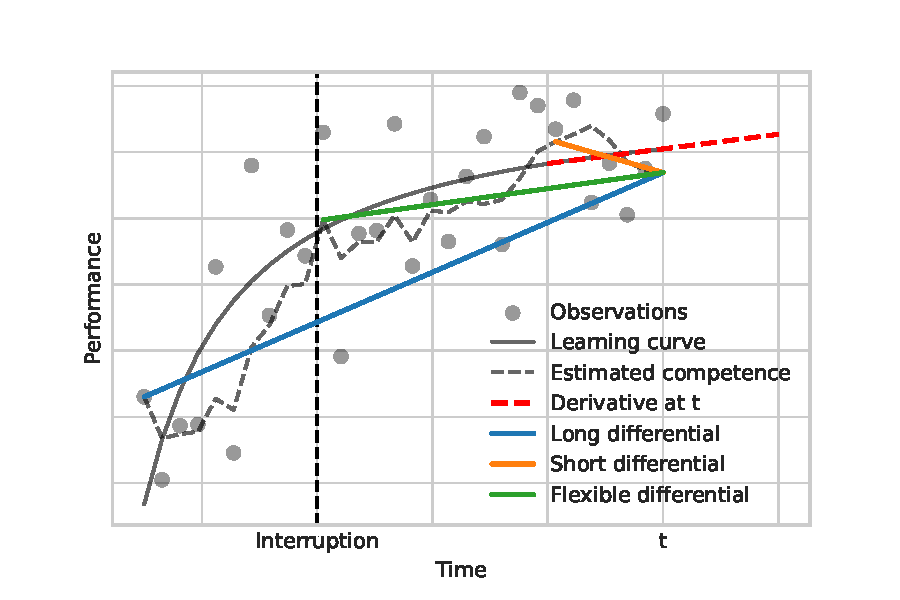
\includegraphics[width=.8\linewidth]{Figures/c5/lptw.pdf}}
    \caption[]{\textbf{Temporal extent of \ac{LP} estimation}. The plot depicts a hypothetical learning curve (blue line), on which performance increases with diminishing returns over time. The derivative of this curve represents the true rate of improvement. The learner does not know the true learning curve or its derivative; they can estimate it by comparing performance outcomes at different points in time (blue dots). Note that learning is interrupted for an unspecified period of time (gray area). Comparing current performance with a very distant reference point is likely to overestimate the derivative (green line). Comparing it to reference points that are too close in time is unreliable, given the noise in observations (red line). Resetting the reference point to the beginning of the current episode is more likely to be accurate, if enough attempts are made during the episode.}\label{fig:5-lptw}
\end{figure}

%This situation is similar to the bias-variance tradeoff in statistics and \ac{ML}. While humans might prefer high-bias and low-variance estimates when it come to predicting uncertain quantities \cite{gigerenzer_heuristics_2011}, a more precise specification would be useful.

% Flexible referencing
Fixed time-window computation might be too restrictive to account for the diversity of learning trajectories across different tasks. Shorter time windows are more useful for easier tasks where learning progresses rapidly, while longer time windows are more appropriate for more slowly developing skills. Fixed time-window computation also requires ad hoc assumptions to handle situations in which the reference point extends beyond what is available. For example, given a time window of size $\tau$, the learner would require at least $\tau$ performance evaluations to compute \ac{LP}, unless the parameter is allowed to vary in the beginning. A more flexible approach would be to reset the reference point to when the task is switched to. This would turn the relationship between \ac{LP} and its temporal extent upside down: instead of \ac{LP} depending on the fixed time window, the temporal extent of \ac{LP} judgments would depend on the rate of learning (assuming that low \ac{LP} signals the need to disengage from the current task). This approach is in line with psychological metacognition literature, namely the \emph{Region of Proximal Learning} theory \cite{metcalfe_region_2005}. This theory proposes that once a task is chosen, the amount of time spent on the task will depend on \ac{LP}, here defined as the contrast between the competence judgment at the beginning of task engagement and the dynamic judgment of competence that changes over the course of task engagement.

% Summary
In summary, I propose to assume that in commonly encountered tasks devoid of clear performance feedback, \ac{LP} computation is based on performance data that learners decide to monitor. Such data may not correspond to our preconceived objective criteria, so it needs to be validated empirically. What measures learners consider is only one piece of a puzzle. To understand \ac{LP} computation more fully, we also need to understand what they compare the monitored measures to. The next section describes an ongoing behavioral study for addressing these issues.

\section{Empirical Study of Improvement Judgments}
One approach to study the computational tenets of metacognitive judgments of improvement is by observing how subjective self-evaluations change over the course of practicing a skill. To increase the ecological validity of the results, we want to emulate a naturalistic learning process which is extended in time, interrupted by other daily activities, and does not feature advanced external performance intel. To meet these demands, we have designed a sensorimotor learning activity presented to participants as a video game, called \emph{Lunar Lander}. The goal of the game is to guide a spacecraft onto a landing platform in a controlled manner, so that it does not crash on impact with the ground or go off-screen. To probe participants' subjective judgments about their performance, we solicit the corresponding verbal reports. The secondary objective of the study is to evaluate the impact of subjective judgments of performance dynamics on the motivation to engage in the task. For this, we employ existing verbal psychometric instruments and behavioral techniques for measuring intrinsic motivation.

\subsection{The Lunar Lander Game}

% Background
The game is based on a famous arcade video game \cite{LunarLander19792021}. Using JavaScript and the Box2D physics engine, we implemented a custom version of the game (see Fig. \ref{fig:5-ll_ss}) in order to control the game difficulty and to be able to record the game play. Like the original, our version features a controllable a spacecraft and a randomly generated uneven terrain (see Figure). The game is played across multiple trials. Within a single trial, there is a constant gravity vector that can point directly downward or be slanted in order to create an impression of constant wind.

\begin{figure}[bth]
    \centering
    {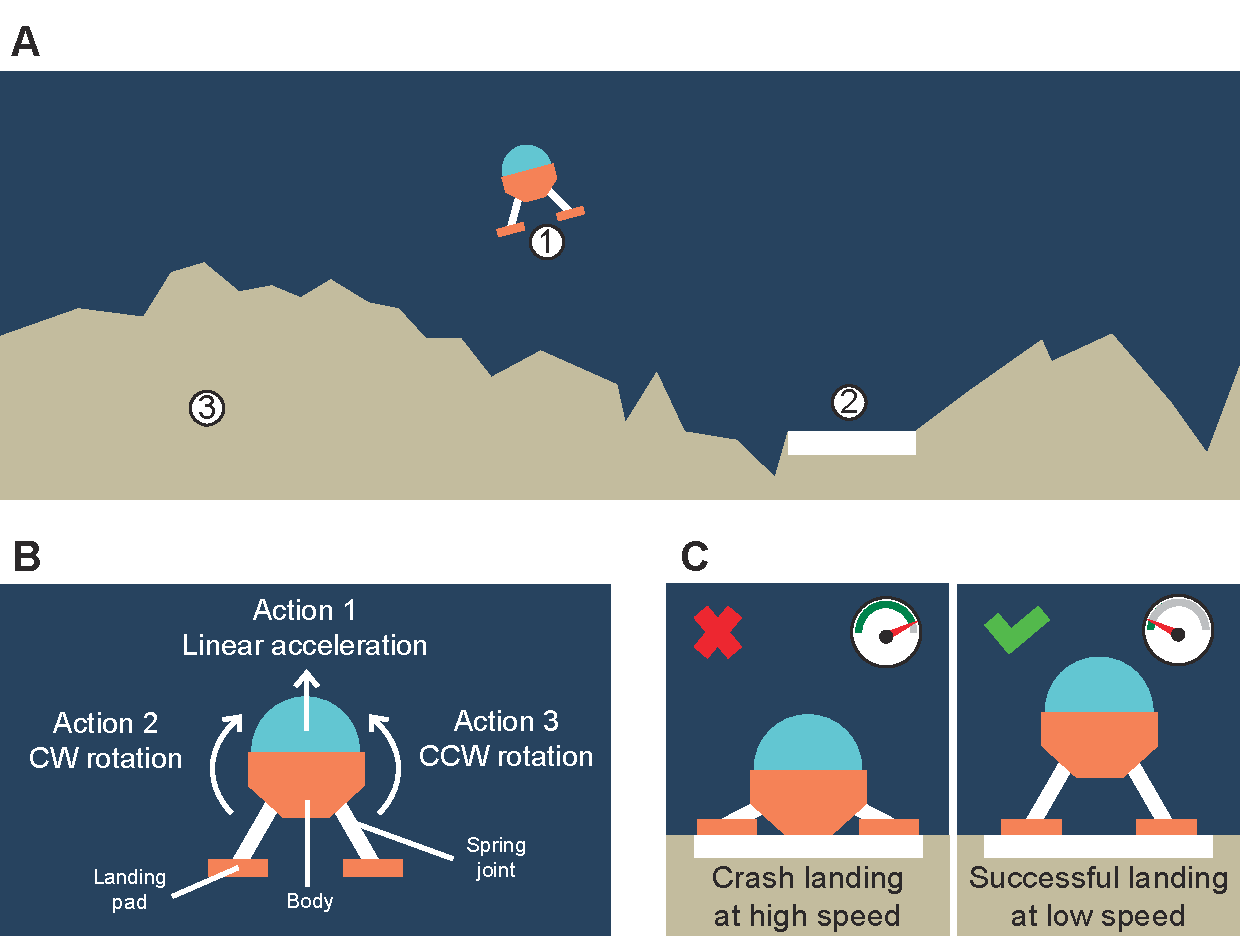
\includegraphics[width=\linewidth]{Figures/c5/ll_ss.pdf}}
    \caption[]{\textbf{The Lunar Lander game}. \textbf{A}, A single frame from a game trial. The spacecraft \circled{1} is controlled by the player to land it onto the platform \circled{2} and avoid crashing into the terrain \circled{3}. The crashing event is triggered whenever the body of the lander (see \textbf{B}) collides with any other object in the environment, including the spacecraft's own landing pads. \textbf{B}, The spacecraft (consisting of the body, two spring joints, and two landing pads) can be controlled by 3 actions: linear acceleration, and clockwise/counterclockwise rotation. \textbf{C}, Successful landing requires placing the spacecraft (landing pads down) at a sufficiently low speed. Even if a player successfully drives the spacecraft to the landing platform, exceedingly high speed causes the spring joints to compress, resulting in a crash.}\label{fig:5-ll_ss}
\end{figure}

% Gameplay
Each trial can end in one of three ways. The spacecraft can go off-screen, in which case, the player is informed that the lander has been lost. The body of the spacecraft can make contact with the ground, in which case is informed that the lander has been crashed. Finally, if the spacecraft can be landed by being carefully placed onto the landing platform (landing pods down) and being kept there for 3 seconds, in which case the player is informed that the lander has successfully landed. The legs of the lander to which the landing pods attach are implemented as spring joints that can be compressed under a force. Thus, the momentum of the spacecraft must be controlled upon landing, even if the spacecraft descends in an upright angle; otherwise the legs will over-compress and the lander will crash.

% Controls
The spacecraft can be controlled by 3 actions (4, if we count doing nothing as an action). Players can rotate the lander clockwise or counter-clockwise and propel it linearly in the direction of the longitudinal axis. Under the hood, actions apply impulse to different points on the spacecraft body. Since there is no friction, stopping or slowing down the angular motion of the body in one direction requires applying an impulse in the opposite direction. Pressing and holding an action key amounts to applying the corresponding impulse on each cycle of the physics simulation, making the spacecraft gain momentum very quickly. Mastering the game requires learning to control the spacecraft, which entails understanding the effects of actions in various contexts. Specifically, learning the game physics requires improving predictions about the velocity of the spacecraft, given the applied actions and the existing momentum.

% Difficulty control: Lander
There are several parameters that determine the difficulty of the game. We can manipulate the rigidity of the leg joints, which determines the speed with which the spacecraft can be landed safely. We can also manipulate the amount of force exerted on the spacecraft by actions. Increasing these forces makes it easy to lose control over the spacecraft, and decreasing them makes the spacecraft very inert and unresponsive. It is also possible to apply noise to actions to simulate control stochasticity.

% Difficulty control: Initialization
In addition to manipulating the lander parameters, we can also control the environment initialization. For example, we can control the initialization distance between the lander and the platform. Traversing more space might be more challenging. We can also change the width of the landing platform, as well as its height relative to surrounding terrain. Finally, we can control the gravity of the environment, parameterized by vertical and horizontal forces on movable objects. By manipulating the horizontal force, we can create a wind effect that drags the lander to one side of the screen and not just downwards. In the pilot study reported below, we experimented with some of these initialization parameters in order to see their effect on average rates of different outcomes.

\subsection{Performance and Improvement Measures}

% A need for scale validation
To measure people's subjective judgments of improvement, we will ask participants to verbally report their feelings on a numerical scale. To the best of our knowledge, no empirically validated psychometric scale for measuring progress judgments exists. Therefore, we will have to design a new scale, which entails some initial experimentation with several items and in order to measure their consistency \cite{kline_psychological_2005,mcneish_thanks_2018}. This can be done in a separate study aimed specifically at engineering an instrument for reliable and valid measurement of \ac{LP}.

% Different kinds of LP
Improvement judgments can be instantaneous and prospective. Instantaneous judgments report how much improvement is experienced by the learner at the time when the judgment is made. In contrast, prospective judgments correspond to feelings of expected improvement, if the task was practiced for some additional period of time. It is not obvious how these kinds of judgments relate to each other and what effect they have on motivation. Therefore, we want to design an instrument with a subscale for each kind of judgment.

% Subjective and objective measures
Although the primary goal is to model instantaneous improvement judgments using objectively observed measures of performance, it would be useful to periodically collect people's subjective judgments of competence, effort, and difficulty. This can be accomplished efficiently by administering (a part of) the NASA-TLX questionnaire \cite{hart_development_1988} several times during practice. NASA-TLX measures 7 components of the task load, including: 
\begin{enumerate}
  \item Mental demand
  \item Physical demand
  \item Temporal demand
  \item Performance
  \item Effort
\end{enumerate}
We will statistically model performance scores using the hypothesized subjective components of competence (see \autoref{subsec:pilot}. Additionally, to get a better idea of what determines instantaneous and prospective judgments of improvement, we will fit regression models of these judgments as a function of combined measures of performance and task load, followed by model comparisons. 

\paragraph{Intrinsic Motivation Measures}

% SIMS
In order to assess the potential effects of \ac{LP} judgments and other subjective/objective measures of performance on motivation, we will use the \acf{SIMS} scale \cite{guay_assessment_2000}. The scale is grounded in Self-Determination Theory \cite{ryan_self-determination_2000,ryan_self-determination_2017} and measures 4 distinct components:
\begin{enumerate}
  \item Intrinsic motivation
  \item Identified regulation
  \item External regulation
  \item Amotivation
\end{enumerate}
The intrinsic motivation component assesses the extent to which an activity is evaluated as interesting, pleasant, and fun. The identified regulation subscale measures the importance of the activity to the individual. The score on the external regulation scale indicates the extent to which the individual feels forced to do an activity (by external forces). Finally, amotivation measures the individual's unwillingness to participate in an activity.

We will also use several subscales of the \acf{MSLQ} instrument \cite{duncan_motivated_2015}:
\begin{enumerate}
  \item Intrinsic goal orientation
  \item Extrinsic goal orientation
  \item Task value
  \item Self-efficacy for learning and performance
  \item Control beliefs
  \item Metacognitive self-regulation
  \item Effort regulation
\end{enumerate}
The first 3 subscales provide additional measures of motivation. The Self-Efficacy subscale can be interpreted as an absolute prospective judgment of improvement -- it reflects the belief that the task can be mastered eventually, time constraints aside. The remaining 3 subscales can be used as control variables to potentially account for some of the variance in performance and improvement judgments. It is possible that above and beyond the monitored performance measures, improvement judgments are associated with certain behavioral tendencies, including believing that effort is meaningless (low control beliefs), not taking control over one's learning (low metacognitive self-regulation), and not persevering in face of challenges or boredom (low effort regulation). It is worth noting that parts of the questionnaire will need to be adapted to our experiment because the original instrument is designed for the classroom setting.

% Free choice measure
In addition to the self-reported measures of motivation, we will incorporate a behavioral measure of intrinsic motivation using the free-choice technique \cite{ryan_self-determination_2000}. After finishing game practice and questionnaires, participants will be offered a free choice between finishing the session or engaging in more game practice. We will then assess the relationship between subjective/objective improvement and their motivation (either acceptance rate or time of additional practice) to engage in the task when they do not have to. 

\subsection{Pilot Study}\label{subsec:pilot}

% Goals of the pilot study
The goals of the first pilot run of our study were (1) to assess the effects of game initialization parameters on task achievement, (2) to explore the relationships between several performance measures and improvement judgments, and (3) to explore the relationships between improvement judgments and motivation.

\subsubsection{Procedure} 
We asked participants ($N=54$) to practice the game over 3 sessions that spanned 5 days. Due to the pandemic caused by COVID-19 outbreak, the pilot experiment was conducted remotely through a custom-designed online platform. We used a fixed schedule for all participants: session 1 was completed on day 1, session 2 on day 2, and session 3 on day 5. Thus, there was 1 day between sessions 1 and 2; and 3 days between sessions 2 and 5. Each session consisted of 3 phases: task practice, questionnaire, and free-choice task (Fig. \ref{fig:5-procedure}). The study was approved by Inria's Operational Committee for the Evaluation of Legal and Ethical Risks (OCELER).

% Experiment procedure
\begin{figure}[bth]
    \centering
    {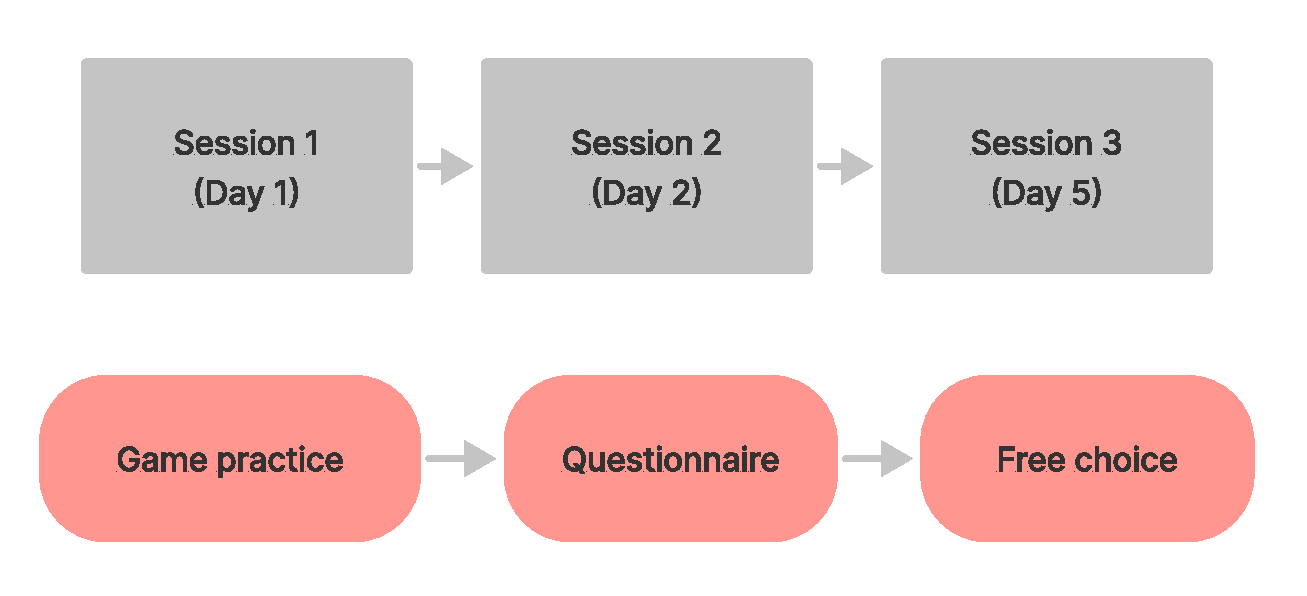
\includegraphics[width=\linewidth]{Figures/c5/procedure.pdf}}
    \caption[]{\textbf{Pilot experiment procedure}. Participants completed 3 sessions, each on a different day (top row). Each session consisted of game practice, followed by a questionnaire, and a free choice task (bottom row).}\label{fig:5-procedure}
\end{figure}

% Two practice durations
Participants played multiple trials of Lunar Lander during the task practice phase. As a precaution from a potential floor/ceiling effect, we asked some participants to practice for 10 minutes, and others for 20 minutes, in each session. In the beginning of each session, participants read through the same instructions about the goal, the rules, and the controls of the game.

% Questionnaire and free choice
After finishing the practice phase, participants were asked to fill in a questionnaire consisting of performance-improvement, NASA-TLX, and \ac{SIMS} questions. \ac{MSLQ} questions were only asked during the second session. After finishing the questionnaire phase, participants were informed that they have finished the session and that they could practice more if they wanted or move on from our task.

\subsubsection{Findings}

\paragraph{Task achievement}

% Success rates across sessions
\begin{figure}[t]
    \centering
    {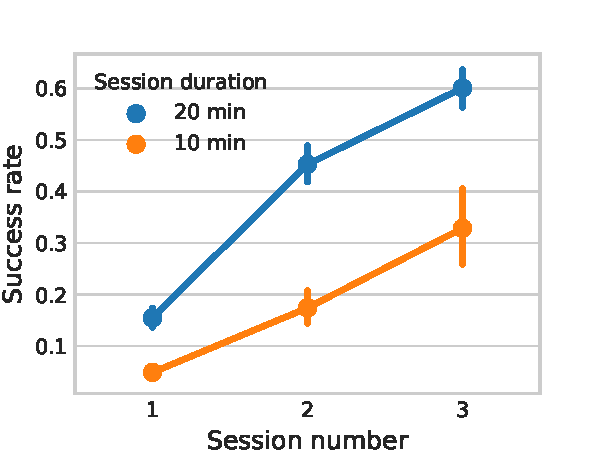
\includegraphics[width=.5\linewidth]{Figures/c5/success_rates.pdf}}
    \caption[]{\textbf{Success rates across sessions and session durations}. The points represent success rates in the 10-minute (blue) and the 20-minute (orange) condition. Error bars show 95\% \ac{CI} (the increasing intervals for later sessions are due to participant dropout). Success rates increased steadily in both 10-minute and 20-minute conditions. More time per session allowed participants to perform better, but performance increased almost linearly with each successive practice session, regardless of the duration. Low levels of success in the 10-minute group suggests a floor effect.}\label{fig:5-success_rates}
\end{figure}

% Effects of time on success rate
To get a general sense for the difficulty of the game, we analyzed the success rates across the three practice sessions for the two session-duration conditions (10 minutes and 20 minutes). We fitted a logistic regression of binary trial outcome (success vs. crash/off-screen) as a function of session duration, session number, and their interaction (setting the 10-minute session 2 as the reference group). As shown in Fig. \ref{fig:5-success_rates}, success rates in 20-minute sessions were higher compared to 10-minute sessions. The logistic model predicted the odds of success in a 20-minute (second) session to be 3.924 times higher compared to a 10-minute (second) session (\ac{OR} $=3.924$, 95\% \ac{CI} $=[3.017, 5.105]$, $z(5, 4654)=10.189$, $p<.001$). Success odds were also significantly different across sessions: compared to the 2nd (10-minute) session, participants were less likely to land during the 1st (10-minute) session (\ac{OR}(5, 4654) $=0.244$, 95\% \ac{CI} $=[0.174, 0.343]$, $z(5, 4654)=-8.137$, $p<.001$) and more likely to land in the 3rd (10-minute) session (\ac{OR}(5, 4654) $=2.32$, 95\% \ac{CI} $=[1.538, 3.505]$, $z(5, 4654)=4.008$, $p<.001$). There was no interaction between session duration and session number, suggesting that participants improved consistently across sessions within each session-duration group. The analysis also advises against restricting the practice to 10 minutes per session, especially for the 1st session. where only about 5\% of all trials were successful. This floor effect might complicate assessing the relationship between performance improvement and subjective judgments of \ac{LP}.  

% Effects of continuous covariates on success rates
\begin{figure}[tbh]
    \centering
    {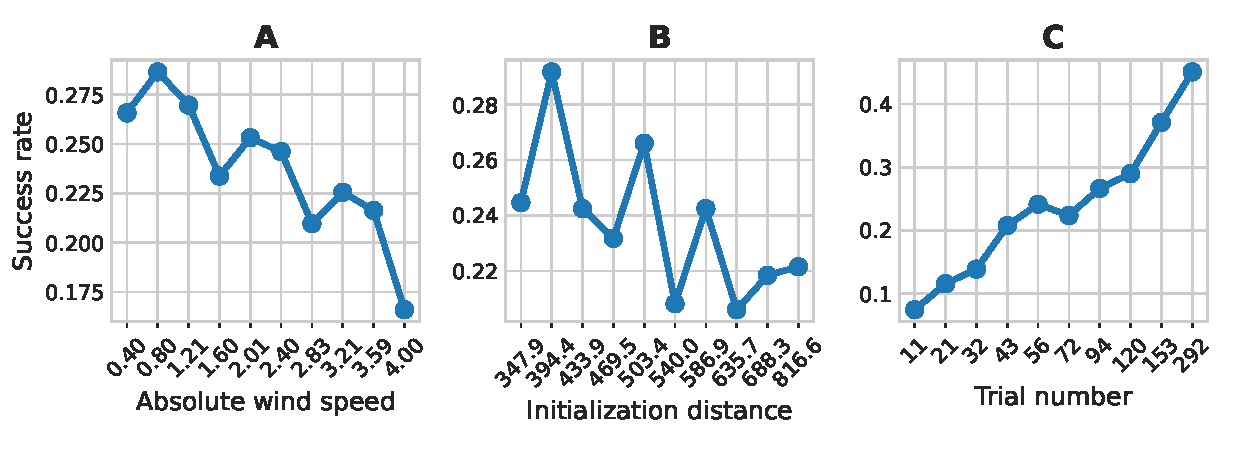
\includegraphics[width=\linewidth]{Figures/c5/init_param_effects.pdf}}
    \caption[]{\textbf{Success rate covariates}. The three panels show the proportion of successful trials across covariate the respective covariates quantized into 10 bins (values on the $x$-axes show quantile upper bounds). \textbf{A} shows the negative correspondence between success rate and the absolute value of the wind parameter. \textbf{B} shows the negative relationship between success rate and initialization distance between the lander and the platform. \textbf{C} shows how average success rates increased over time across sessions. In the range of the first 300 trials, the population-level success rate appears to be increasing linearly with the number of attempts.}\label{fig:5-init_param_effects}
\end{figure}

% Wind and initialization distance
Next, we looked at the effects of game initialization parameters on success (see Fig. \ref{fig:5-init_param_effects}). We fitted a logistic regression of trial outcome as a function of two initialization variables: the absolute wind speed and the initialization distance to the platform; we also included the trial number (cumulative across sessions) as a control variable. To compare the effects, we standardized the regression coefficients by $z$-scoring the covariates. We only included trials from participants who had at least one successful attempt across all sessions played. All three predictors had coefficients significantly different from zero. Thus, accounting for the increasing odds of success over time (\ac{OR} $=1.627$, 95\% \ac{CI}$=[1.518, 1.743]$, $z(3, 3623) = 13.871$, $p = 001$), participants were less likely to land under a stronger wind (\ac{OR}(3, 3623) $=0.821$, 95\% \ac{CI}$=[0.762, 0.884]$, $z(3, 3623) = -5.249$, $p<.001$) and when initialized farther from the target (\ac{OR}(3, 3623) $=0.882$, 95\% \ac{CI}$=[0.819, 0.949]$, $z(3, 3623) = -3.339$, $p<.001$). These results present empirical validation for the predicted relationship between the two game-initialization parameters and task difficulty.

\paragraph{Judgments of improvement}

% JOLD questions
At the end of each game-practice session, we asked participants several questions about their subjective improvement. One question probed the retrospective improvement judgment: "Rate how much your current level of performance has changed \textit{compared to the beginning of today's session}". Participants responded by moving an interactive slider along a discrete 11-point semantic differential scale ranging between two polar response categories: "Much worse" (-5) and "Much better" (5); putting the slider at the center of the scale was assumed to indicate the reporting of no perceived change in performance. The same response scale was used to yield a prospective improvement judgment, prompted by "Rate how much you expect to improve over the next session". We explored how self-reported feelings of retrospective and prospective improvement related to different aspects of performance.

% Correlation between prospective and retrospective judgments
\begin{figure}[bth]
    \centering
    {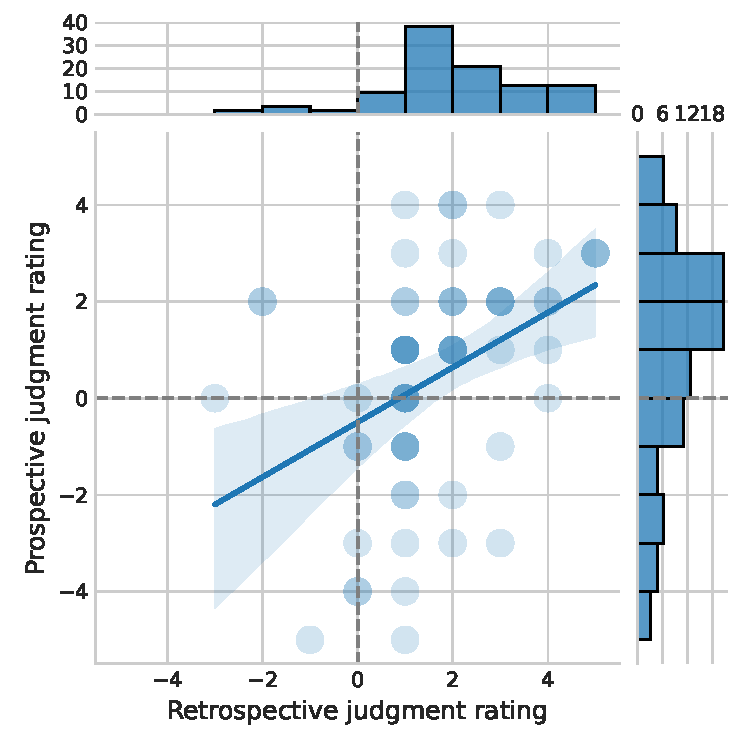
\includegraphics[width=.6\linewidth]{Figures/c5/jolds_corr.pdf}}
    \caption[]{\textbf{Retrospective and prospective judgments}. The central panel shows the joint distribution of retrospective and prospective improvement judgments. Darker circles indicate the greater amount of overlapping data points. The line represents a fitted linear regression of prospective judgments on retrospective judgments (the shaded area shows the 95\%\ac{CI} for the model) The marginal histograms show relative frequencies (\%) of self-reported scores.}\label{fig:5-jolds_corr}
\end{figure}

% Relationship between retrospective and prospective judgments
Fig. \ref{fig:5-jolds_corr} shows the joint sample distribution between retrospective and prospective improvement judgments. There were a total of 63 observations (22 out of 85 prospective-improvement judgments were lost due to data collection error). The marginal histograms show that improvement judgments were mostly positive. However, subjects seemed less optimistic about their future improvement, compared to how they thought they had previously improved, as indicated by a longer tail into the negative range of the prospective judgment scale. Spearman's correlation coefficient between prospective and retrospective judgments was moderate and significantly different from 0 ($r_{\mathrm{Spearman}}(61) = .491,\ p < .001$). Thus, retrospective feelings of improvement seem to explain some of the variance in prospective progress judgments.

% Idea 1: JOLDs ~ incrase in success rate
Next, we investigated several hypothesized behavioral predictors of improvement judgments. We started with a simple competence indicator -- the change in rate of externally provided positive feedback. Namely, each trial could end by either successfully landing the spacecraft or failing to do it. Dividing the number of successful landings by the total number of trials attempted gives us the success rate. For each subject and for each session, we calculated the success rate in the first and the second half of the session and then subtracted the latter from the former (a positive difference indicates improvement). Fig. \ref{fig:5-jolds_and_srd} depicts the relationships between retrospective and prospective improvement judgments (respectively) and the change in success rate in the corresponding session. Increasing rates of success predicted the retrospective improvement judgments, but not the prospective improvement judgments (see legend to Fig. \ref{fig:5-jolds_and_srd}).

% Improvement and success rate difference
\begin{figure}[bth]
    \centering
    {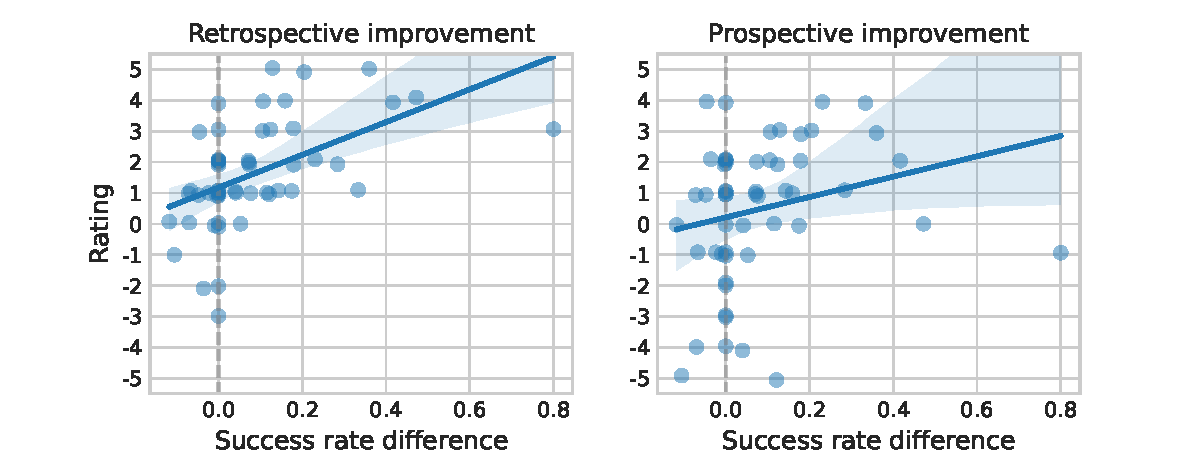
\includegraphics[width=\linewidth]{Figures/c5/jolds_and_srd.pdf}}
    \caption[]{\textbf{Increasing success rate predicts self-reported past improvement, but not the expected future improvement}. The circles represent individual data points. Small uniform jitter was added to the rating values for presentation purposes. The lines represent linear regression models of retrospective and prospective improvement ratings, respectively. The shaded regions represent 95\%\ac{CI} for the models' predictions. Objective performance improvement, indexed by increasing success rates, reliably predicted the retrospective judgments (slope $=5.805$, 95\% \ac{CI}$=[2.96, 8.649]$, $t(1, 73) = 4.066$, $p<.001$) but not the prospective judgments (slope $=3.301$, 95\% \ac{CI} $=[-0.581, 7.183]$, $t(1, 52) = 1.706$, $p=.094$).}\label{fig:5-jolds_and_srd}
\end{figure}

% Why look at other performance measures
Strikingly, however, 14 out of 46 participants ($30.43\%$) reported positive improvement in the absence of a single successful attempt\footnote{We report the results from 46 (not 54) participants, because 8 out of 54 participants dropped out immediately after completing the 1st game practice without filling in the questionnaires.}. This could be interpreted in at least two different ways. One possibility is that people base recent improvement judgments on success-rate dynamics, but self-reported ratings of improvement are unreliable due to metacognitive miscalibration. Another explanation is that improvement self-reports are based on something other than task-achievement feedback. One of the motivations behind studying verbal reports of subjective improvement was to examine whether people can accurately self-assess. However, to study metacognitive accuracy -- the covariance between subjective and objective improvement -- we need to choose valid objective measure(s). Previous research seems to present conflicting conclusions regarding the role of external competence feedback \cite[e.g.,][]{townsend_judgments_2011,leonard_young_2021}, but there is evidence to suggest that people do attend to task-relevant competence measures when binary feedback is not available \cite{locke_performance_2020}.

% Introducing continuous objective game variables
In our version of the Lunar Lander game requires continuous optimization of 3 controllable variables: the distance between the landing platform and the lander, its speed and its angle. These variables are mutually constraining, and their optimal values depend on the situation: for example, higher speeds and more horizontal angles are better in the beginning of an episode when the lander is far away from the target, but lower speeds and more upright angles are better when the lander is close to the target. We measured the $(x,y)$-position of the spacecraft in each animation frame, which allowed us to calculate approximate lander speed and distance to the platform, but not the angle  (which should be measured in future research).

% Sanity check of the objective variables: Explaining the figure
To check our intuition that competent performance requires an optimization of speed and distance, we plotted these variables across time (Fig. \ref{fig:5-dist_speed_start_800_CI99}. Interestingly, the first few frames of a trial seems to be enough to predict whether the trial will be successful or not. Fig. \ref{fig:5-dist_speed_start_800_CI99} shows that on successful trials, participants are able to drive the lander closer to the target sooner by increasing speed at a slightly higher rate (this is especially clear from the bottom right panel). Moreover, when successful, participants are more efficient at dropping the speed after the initial acceleration.

. Presumably, participants use some characteristics of lander movement trajectories in order to evaluate their performance. 
Fit polynomial models of `distance ~ time`. Find mean coefficient values for successful trials across all participants (maybe divide by whether trial begins far or close). Then for each trial, compute the distance between trial-fitted coefficients and the prototypical success coefficients. See if the slope of this distance-to-competence accounts for JOLD judgments (controlling for success rate).

% Speed and distance across time
\begin{figure}[bth]
    \centering
    {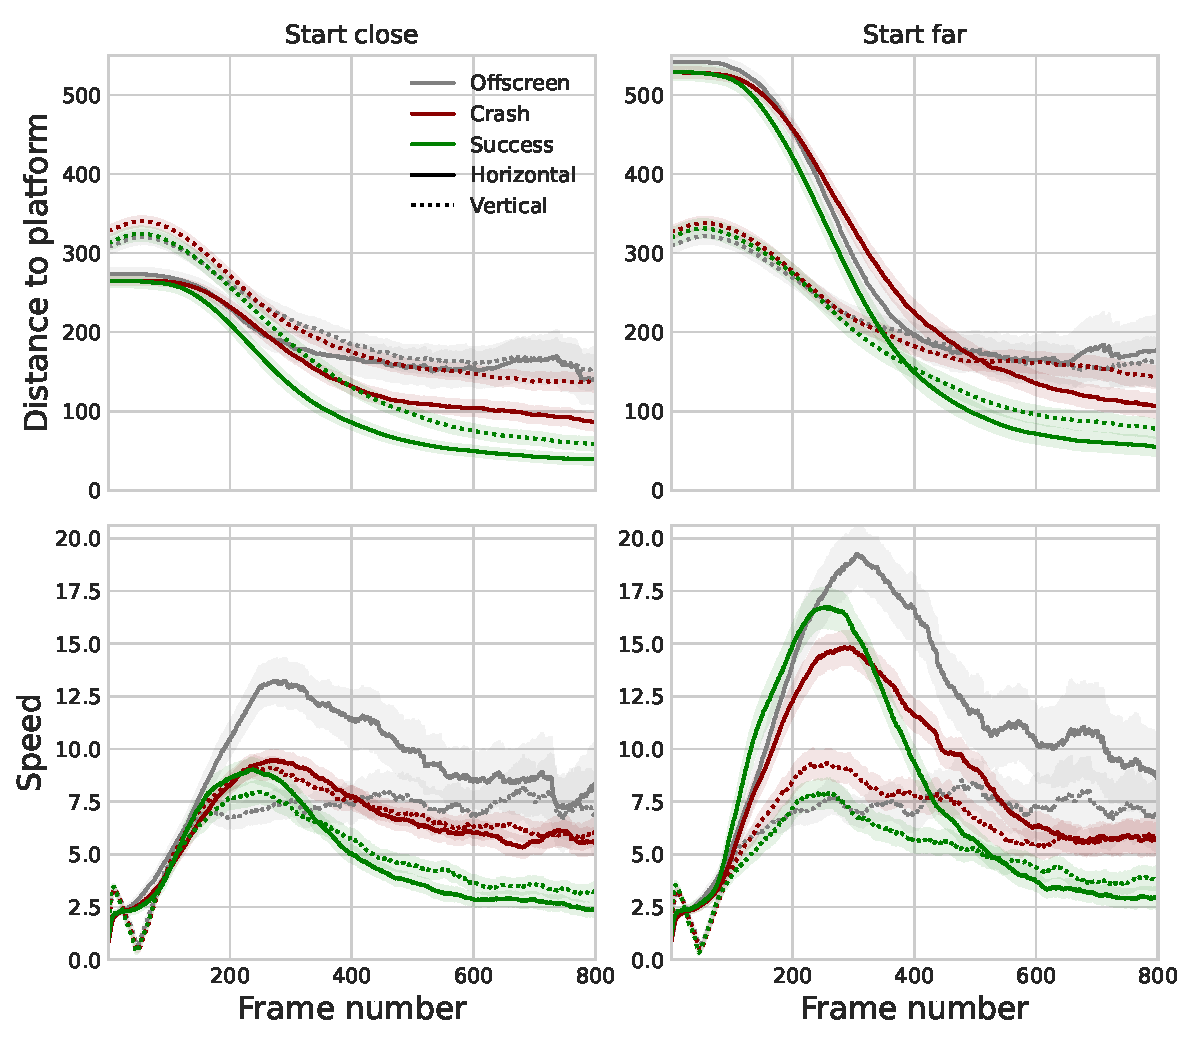
\includegraphics[width=\linewidth]{Figures/c5/dist_speed_start_800_CI99.pdf}}
    \caption[]{\textbf{Continuous performance indicators in the beginning of a trial}. To produce this figure, we grouped all trials according to the final outcome (success, crash, offscreen). In each group of trials, we averaged the two variables along each frame of the trial. Since trial durations varied considerably, we used only the first 800 frames of each trial to produce the figure. The missing frames from trials shorter than 800 frames were omitted from calculations of the mean (hence the wider 99\%\acp{CI} for later frames). Distance and speed trajectories for trials on which the lander was initialized closer and farther from the target are shown in separate columns. The top row shows how players controlled the Euclidean distance to the platform over in the beginning of the trial. The bottom row shows the evolution of speed, defined as the absolute difference between position coordinates from one frame to the next. Colors indicate trial outcomes; line styles indicate spatia dimensions. \textit{Note:} the exact frame-rate was not recorded, since it depended on the specifications of participant's personal devices.}\label{fig:5-dist_speed_start_800_CI99}
\end{figure}


% Idea 3: JOLDs ~ trial_mean_speed_slope

% Idea 4: JOLDs ~ success_rate_slope + wad_slope + trial_mean_speed_slope

\subsection{Discussion}

% How can learning dynamics be evaluated objectively? To get started, consider an analogy with classical mechanics. In classical mechanics, objects are characterized by their position measured in some coordinate system (which can be 2D or 3D, for example). Object position provides an instantaneous description -- a snapshot -- of the object. Velocity is the first-order temporal derivative of position and it describes how position changes per an infinitesimally small unit of time. 

% Analogously, we can think of a subject's instantaneous level of competence that varies with time. Instantaneous competence provides a snapshot of one's ability while the temporal derivative of instantaneous competence describes how it evolves over an arbitrarily small unit of time. If $x = f(t)$, then $f'(t) = \frac{dx}{dt}$. In words, if competence ($x$) is a function of time ($t$), then the temporal derivative of competence is the rate of change in competence over an arbitrarily small unit of time. 

% :::info
% Note that it is not necessary to know the mathematical form of $f(t)$ in order to get $f'(t)$ if all we care about is the numeric value of the derivative at $t$. Knowing the precise functional form is only necessary if the one wants to obtain the true derivative $\frac{dx}{dt}$, where $dt$ is an infinitesimally small. It is unlikely that humans track such minute temporal changes. Numerical approximation of this quantity for an arbitrary differential $\bar{dt}$ is simple: one just needs to compare the value of $x$ at time $t$ with $x$ at $t - dt$.
% :::

% The computation of a temporal derivative is essentially symbolic. That is, to carry it out, the computer (that who/which computes) must represent the dynamic quantity (e.g., competence) symbolically as time-series. In numerical approximation of the temporal derivative, the time differential itself has a symbolic representation. At this point, we can assume that our minds indeed perform such symbolic computations in order to produce JOLDs. This would mean that objective evaluation of progress is no different to the actual cognitive process, except that the latter might be carried out implicitly (i.e., unconsciously). Let's put this possibility aside and move on to another one, which, I feel, is better connected to other cognitive theories of learning (which is desirable in science, right?).

% ### Progress as a meta-learning process
% It is possible to imagine a mechanism that computes competence changes without any explicit symbolic representations. Knowledge gains can be indexed by the very change of the underlying sensorimotor learning system itself, as opposed to explicit computation and comparison of competence levels at different points in time. Different levels of change in the sensorimotor learning system might correspond to distinct neurochemical (or backpropagational) states that might represent progress for other cognitive systems downstream, e.g., for the linguistic system to generate verbal report and for the executive systems to guide attention/task engagement.

% To illustrate, imagine how a simplified sensorimotor system might learn from prediction errors (see Figma diagram below, which is inspired by [Reinforcement Learning](http://incompleteideas.net/book/the-book.html) and [Control Theory](https://www.researchgate.net/publication/2431469_Computational_Aspects_of_Motor_Control_and_Motor_Learning)). The process begins with a selected goal, e.g., to land the lander. Upon perceiving sensory context coming from the environment at time $t$, the system equipped with prior knowledge (internal inverse model) takes a series of actions to reach the goal. An efferent copy of the action(s) enters the internal forward model that predicts outcomes of the action(s) taken. The performed action(s) creates the next environmental state (at time $t+1$) which is picked up by the system as action(s) effect. This effect can then be used to update the system's two internal models:
% 1. The forward model is updated by a contrast between the sensed state (the effect) and the predicted state. Learning results in better predictions of the next states from actions and contexts.
% 2. The inverse model is updated by a contrast between the sensed (affected) state and the goal. Learning results is choosing better the actions to achieve selected goals.

% {%figma https://www.figma.com/file/SoF0Lhp7fmSZdWxCYsWvzR/Full-learning-loop?node-id=0%3A1 %}

% This highly simplified example of a sensorimotor learning system illustrates that the learning-progress signal does not need to depend on a symbolic computation of competence derivative (although it could, as I discuss below). Instead, the amount of learning progress scales with how much the subjective internal models themselves change. Note that there might be multiple sources of progress, if the existence of separable forward and inverse models is assumed.

% ### Progress as changing beliefs
% Another possible mechanism that allows to track learning progress without relying on symbolic differentiation involves explicit beliefs about the system's own abilities (collectively called "self-efficacy"). Here, we assume that the cognitive system features a so-called self-efficacy model that, given a goal, can output the subjective likelihood of achieving it. The goal-related outcome, representation of which is derived from sensed effects, can then be used to update the prior beliefs about goal-achievement capabilities of the agent. The amount by which this belief changes can also, in principle, inform the system's competence progress.

% It should be noted that "goals" are underspecified in this discussion. It would be great to have a productive conversation with anyone willing about how goals might be represented in our task. For instance, goals can be represented as categorical criterion (*landed* vs *not landed*) or by a continuous one (average distance to platform). A goal can be even more abstract than that: e.g., *to control the lander well enough to land it at will*.

% ### Critical review of tentative mechanisms

% In summary, I've discussed 3 ways to compute learning progress:
% 1. **Meta-learning**, where learning progress corresponds to the size of the update of an internal model (or some index of the size of the update).
% 2. **Belief-updating**, where learning progress corresponds to the size of the update of a self-efficacy model.
% 3. **Symbolic differentiation**, where learning progress corresponds to the result of symbolic differentiation of an arbitrary quantity, $x$.

% Next, I provide some "armchair" justifications for why it is useful study the belief-updating approach (as we will do in the Lunar Lander experiment) first.

% #### Meta-learning vs Belief-updating

% Mechanisms based on meta-learning and belief-updating do not seem incompatible with each other. The forward and inverse "meta-learning" and the "belief-updating" processes all compute different kinds of learning progress. Good internal-models constitute knowledge of either what happens following one's actions (forward model) or what actions to take in order to achieve a goal (inverse model), while a good self-model constitutes accurate knowledge of one's task-specific aptitude. Improvement of each of these models, then, is of a different kind.

% Knowing *whether* one can achieve something is not necessarily the same as knowing *how* to achieve it[^7]. There are cases where people's explicit beliefs about their abilities and their actual abilities diverge. One prominent example comes from a neuropsychological subject, known as [HM](https://en.wikipedia.org/wiki/Henry_Molaison), who lost his ability to form new declarative memories after a bilateral medial temporal lobectomy. HM, however, was able to retain a visuomotor skill that he acquired post-surgery ([Squire, 2009](https://www.ncbi.nlm.nih.gov/pmc/articles/PMC2649674/)). While HM's internal sensorimotor model clearly improved over time, he never remembered ever performing the task in the past ([Milner, 1965](https://www.semanticscholar.org/paper/Visually-guided-maze-learning-in-man%3A-effects-of-Milner/66a3ce58895d8ddab293e2412eb7616555f867f7)). Presumably, he never knew *whether* he could perform the visuomotor task, yet he knew (implicitly) *how* to do it. 

% Follow up studies of HM's learning abilities showed that he could adapt his behavior in multiple other contexts ([Corkin, 2002](https://www.nature.com/articles/nrn726)), suggesting that human memory is comprised of multiple distinct subsystems. Although a few learning mechanisms are common to many of these subsystems, some of them involve idiosyncratic neurochemical processes ([Bisaz et al., 2014](https://www.researchgate.net/publication/266746974_The_Neurobiological_Bases_of_Memory_Formation_From_Physiological_Conditions_to_Psychopathology)). This taxonomy of learning systems is based on types of memory ([Squire & Zola, 1996](https://www.pnas.org/content/93/24/13515)) and it can be distinguished form a functional distinction between two Complementary Learning Systems (CLS, [Kumaran et al., 2016](https://www.psychologie.uzh.ch/dam/jcr:83bd242c-50a5-45df-919e-3c134ff6979e/Kumaran.TiCS.2016.pdf)). 

% In light of this complexity, it seems unlikely that the brain has evolved several specific metacognitive mechanisms to monitor each learning system within the brain. Belief updating provides a general mechanism for evaluating one's knowledge. Since the goodness of knowledge can be assessed by specific tasks (i.e., tests), beliefs about the relevant goal-achievement capabilities can serve to track the quality of knowledge in a general way. Although the possibility of one or more specific metacognitive mechanisms is not entirely zero, this reasoning provides a reason for investigating mechanism(s) based on belief-updating.

% #### Belief-updating vs symbolic differentiation

% Next, I want to contrast the computation of learning dynamics through symbolic differentiation with the belief-updating mechanism. Unlike in the symbolic differentiation approach, computation of progress in the belief-updating process is implicit (not explicit). Here, progress is a by-product of the evolving self-efficacy beliefs.

% I already discussed another distinction between these mechanisms: JOLDs borne out of belief-updating do not rely on a time-differential. Therefore, a symbolic differentiation account of progress computation makes an ontological claim regarding the existence and involvement of a temporal differential, which has to be rationally justified and empirically validated. This is another reason why I think we can narrow down the scope of our study to focus on the belief-updating approach.

% Nevertheless, some version of what we might call symbolic differentiation is arguably present in human brains, but I believe it is not an integral part of the motivational system that guides task selection and task engagement universally. Symbolic differentiation is likely to be a part of a more general quantitative reasoning system capable of comparing arbitrary quantities. People may accurately answer questions about their JOLDs concerning different time windows by reasoning about their evolving ability[^9] *even if* other special-purpose, progress-evaluating mechanisms are implemented. And even though it might in fact influence one's task engagement, I don't think young children and even adults habitually engage in such quantitative reasoning practices.

% ::: info
% In summary, let me reiterate that I think that we should focus on the belief-updating mechanism in our study. Here is why:
% - There is an established tradition to model belief updating as a computation of the posterior distribution by Bayes rule.
% - Bayesian surprise operationalized as KL divergence has been shown to attract human attention ([Itti & Baldi, 2009](https://www.sciencedirect.com/science/article/pii/S0042698908004380); [Poli et al., 2020](https://advances.sciencemag.org/content/6/39/eabb5053)).
% - An investigation of mechanisms based on internal-model learning is beyond the scope of our study, because of the following reasons:
%     - We don't have a way to measure the learning signal of internal models.
%     - We don't have a good idea of which of many learning systems in the brain the meta-learning system is likely to monitor.
% - Symbolic differentiation is likely to be a general and acquired skill of quantitative reasoning, so does not seem to be an integral part of the motivational system (although it might influence motivation).
% :::

% ## Computational bases of subjective competence

% **We do not have a definitive idea of the nature of subjective beliefs about one's competence**.

% Luckily there is helpful work that provides some clues. [Martí et al. (2018)](https://www.researchgate.net/publication/327067047_Certainty_Is_Primarily_Determined_by_Past_Performance_During_Concept_Learning) found that confidence on a categorization task depends on response accuracy. Participants learned the meaning of a novel concept by trying to classify randomly drawn stimuli as positive or negative examples of that concept. After each guess, they received binary feedback from the experimenters. The authors found that self-reported confidence in understanding the concept (and thus, in providing correct categorization responses) depends on the amount of positive feedback received in the 5 most recent guessing attempts. From the conclusions of this study, we can predict that **subjective competence depends on a binary goal-achievement signal**. The more one succeeds in accomplishing the task -- that is, in landing the lander -- the more one feels competent.

% One problem with this conceptualization is that so long as the player fails to land, he or she is not expected to experience any changes in subjective confidence. However, people can believe that they are getting closer to landing the lander even without ever landing it. What signal might people use to evaluate their competence in the absence of positive reinforcement brought by goal achievement?

% [Locke et al. (2020)](https://shannonlocke.github.io/articles/Locke2020_sensorimotorConf.pdf) studied this question using a sensorimotor task. Specifically, they were interested in what determines humans' explicit subjective confidence judgments on a cloud-tracking task that did not provide binary feedback. The authors present evidence supporting the idea that instantaneous sensorimotor confidence[^2] depends at least partially on goal-based performance monitoring, operationalized as continuous tracking error. This was evident in the association between binary subjective confidence judgments and the temporally proximal tracking error levels.

% Notably, they did not rule out the possibility that other components, such as perceptual certainty and motor awareness, might also contribute to sensorimotor confidence[^3]. The effects of perceptual certainty, motor awareness, and performance error should all be random in our study, since we did not manipulate any these variables. **However, we are specifically interested in whether temporal derivatives of ++performance errors++ are correlated with JOLD reports**. Should we find no association, we will probably need to somehow control for the perceptual and motor factors in order to see the effect of performance error rates. On the other hand, should we find an association between errors and judgments, we can affirm that either (1) the motor and perceptual effects are not present or (2) that the effect of errors is strong enough to be detected despite the noise of the other two factors.

% We can check empirically if performance errors similar to those in Locke et al. (2020) are related to competence judgments collected through one of the NASA-TLX items. We can even go a step further and try to replicate the recency effect reported in their study by which recent performance errors predict competence judgments better than older errors.

% ::: success
% **Hypothesis** : Self-reports of competence (NASA-TLX) are negatively correlated with performance errors.
% :::

% It is easier to think of positive relationships, so instead of performance error, we will use the game score which is a direct opposite of error. To calculate the score, we will first derive a measure of average weighted distance (WAD) to the platform. This is simply the average across game frames of distances between the lander and the platform, where we weight each frame linearly, so that the weight at the end of the trial is 1 and the weight at the beginning of the trial is 0. 

% When WAD is low, it means that for most of the episode the lander was close to the target. When WAD is high, it means that the lander did not spend a lot of time near the target. This measure is similar to what Locke et al. (2020) used, but we shall tweak it a little in order to account for the trial outcome. High values of WAD are good if the player lands successfully because it means that the landing took little time. However, if one fails to land, lower WAD is better than higher WAD because lower values indicate that the lander was closer to the target on average (e.g., one was close to landing but failed at the end).

% Thus, we can operationalize performance score, $s$, as follows:

% $$s = \left\{ 
%   \begin{array}{ c l }
%     \textsf{WAD} & \quad \textrm{if landed} =1 \\
%     -\textsf{WAD} & \quad \textrm{otherwise}
%   \end{array}
% \right.$$

% This score combines both the binary outcome and the outcome-related continuous variable[^10]. We can relate it to the probabilistic confidence variable using the logistic function. Thus, competence, $c$, can be expressed as:

% $$
% c = \frac{1}{1+e^{-s}}
% $$

% Each trial, the player received new data which can be used to updated the belief about his or her competence:

% $$
% c = P(\mathrm{land=1} \mid D) \propto P(D \mid \theta) * P(\theta)
% $$

% <!--  
% ==**Control**== (interesting idea, but we cannot address it in the pilot study).
% ::: spoiler
% *Presumably*, positive competence judgments can be generated even when empirical goal-achievement rate is 0. For example, one can feel more competent than someone else in landing the lander even without ever landing it. One can even feel more competent that the next person without minimizing the error. These possibilities are not captured by achievement-based and error-based competence.

% It might be possible that **subjective competence judgments track the ability to *control* the state of the system**. We can base a measure of control on the concept of *empowerment*, which originates in AI ([Salge et al., 2012](https://arxiv.org/abs/1310.1863)). If we measure entire sequences of people's actions and lander trajectories, we can define control formally as the mutual information between the distributions of actions and sensory effects. We might discover that subjective competence depends on feelings of control.
% :::



% "Reconceptualizing novelty, complexity, and ambiguity in terms of metamemory rather than stimulus features has broken new ground in the study of curiosity’s determinants (e.g., Metcalfe et al., 2017), and helped guide new work on the underlying reward mechanisms involved in curiosity based on the methods of contemporary affective neuroscience (e.g., Gruber et al., 2014)" (Litman, 2019, p. 433).



